%%%%%%%%%%%%%%%%%%%%%%%%%%%%%%%%%%%%%%%%%%%%%%%%%%%%%%%%%%%%%%%%%%%%%%%%%%%%%%%
%
% Evaluation
% 
%%%%%%%%%%%%%%%%%%%%%%%%%%%%%%%%%%%%%%%%%%%%%%%%%%%%%%%%%%%%%%%%%%%%%%%%%%%%%%%


\chapter{Results}
\label{sec:results}

\section{Results}

\newpage

\begin{figure}[H]
\centering
\subfloat[1]{
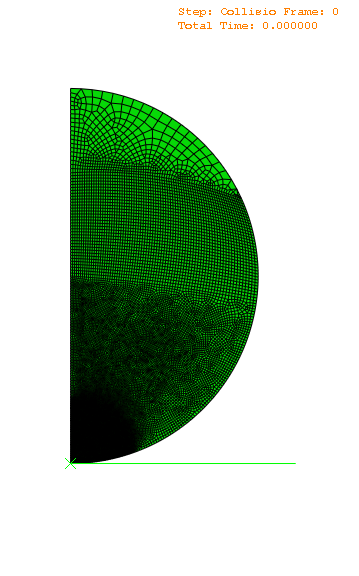
\includegraphics[width=0.25\textwidth]{../images/motion/1.png}
\label{fig:motion1}
}
\subfloat[2]{
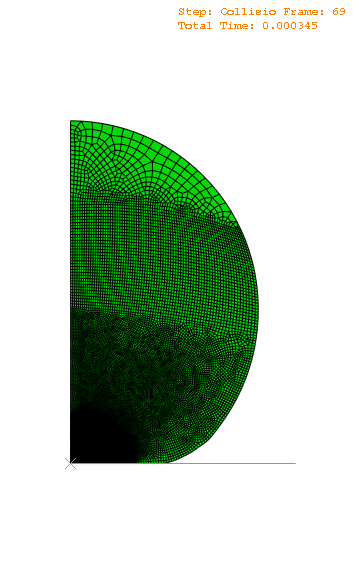
\includegraphics[width=0.25\textwidth]{../images/motion/2.png}
\label{fig:motion2}
}
\subfloat[3]{
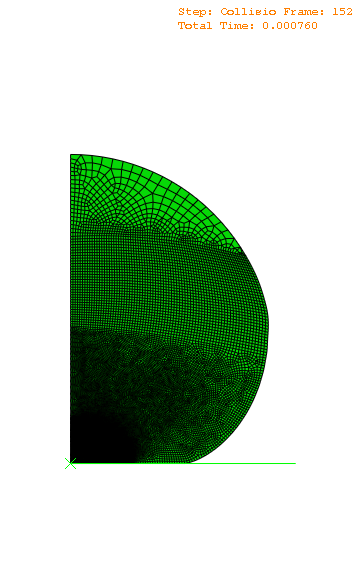
\includegraphics[width=0.25\textwidth]{../images/motion/3.png}
\label{fig:motion3}
}
\subfloat[4]{
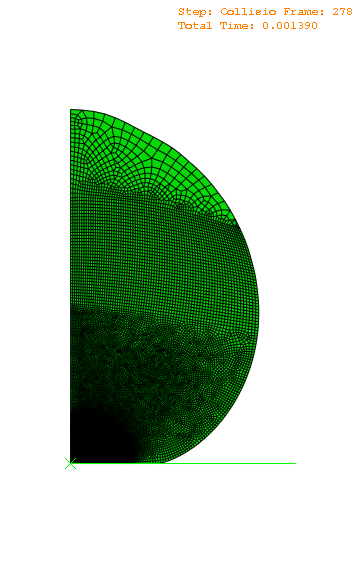
\includegraphics[width=0.25\textwidth]{../images/motion/4.png}
\label{fig:motion4}
}

\subfloat[5]{
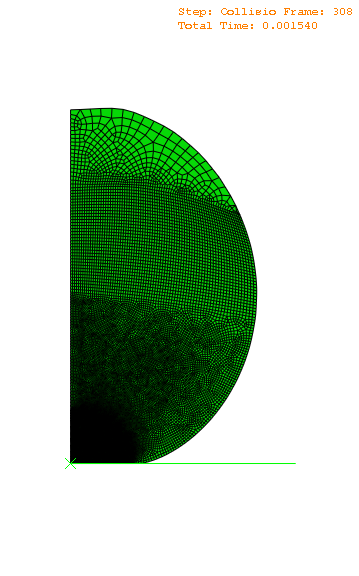
\includegraphics[width=0.25\textwidth]{../images/motion/5.png}
\label{fig:motion5}
}
\subfloat[6]{
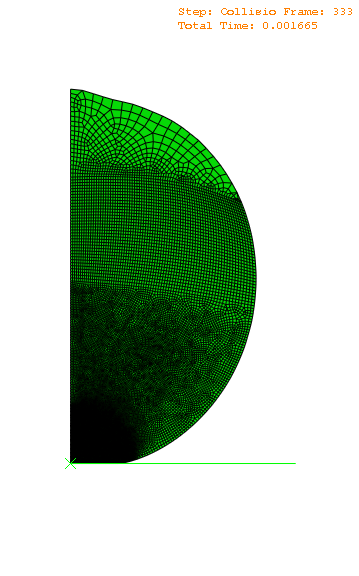
\includegraphics[width=0.25\textwidth]{../images/motion/6.png}
\label{fig:motion6}
}
\subfloat[7]{
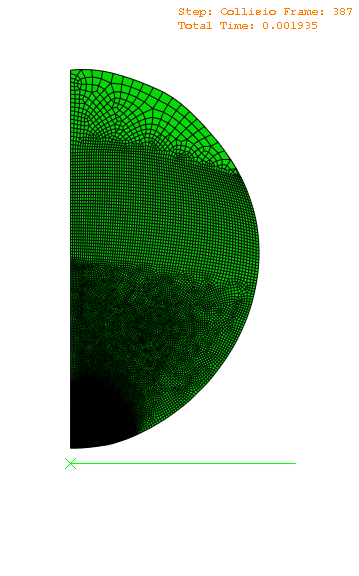
\includegraphics[width=0.25\textwidth]{../images/motion/7.png}
\label{fig:motion7}
}
\subfloat[8]{
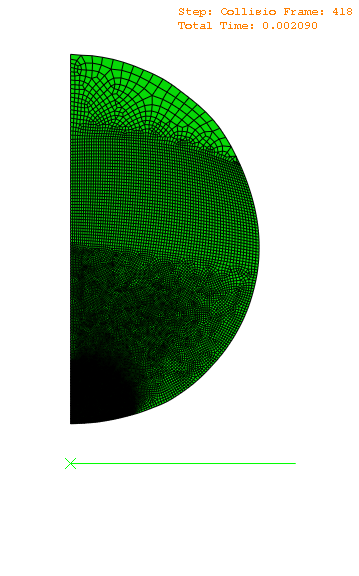
\includegraphics[width=0.25\textwidth]{../images/motion/8.png}
\label{fig:motion8}
}

\subfloat[9]{
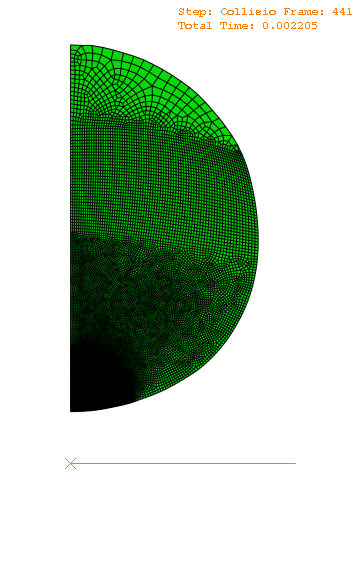
\includegraphics[width=0.25\textwidth]{../images/motion/9.png}
\label{fig:motion9}
}
\subfloat[10]{
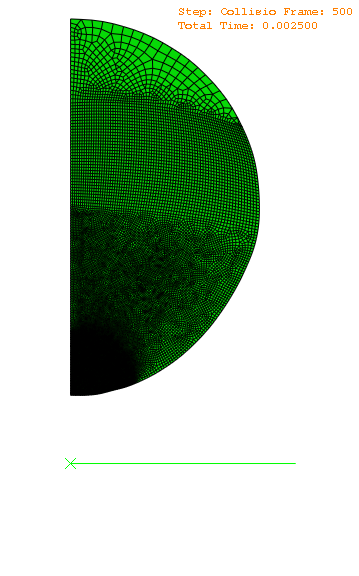
\includegraphics[width=0.25\textwidth]{../images/motion/10.png}
\label{fig:motion10}
}
\label{fig:motion}
\end{figure}

As we study the loss of kinetic energy to vibrations let's first consider a very soft material. The series of figures in \ref{fig:motion} shows the trajectory of a very soft material with $Young Modulus(E) = 6 MPa$ with an impact velocity of $5m/s$. After the contact is lost, spheres starts to vibrate violently. This shows that some part of the kinetic energy possessed by the sphere is converted to strain energy which then caused the vibrations in the sphere. 




%%%%%%%%%%%%%%%%%%COM%%%%%%%%%%%%%%%%%%%

\subsection{Deformation}

\begin{figure}[H]
\centering
\subfloat[Velocity 0.01m/s]{
\includegraphics[width=0.55\textwidth]{{../images/deformationVStime/Velocity1.0}.png}
\label{fig:def1}
}
\subfloat[Velocity 0.10m/s]{
\includegraphics[width=0.55\textwidth]{{../images/deformationVStime/Velocity10.0}.png}
\label{fig:def10}
}

\subfloat[Velocity 0.20m/s]{
\includegraphics[width=0.55\textwidth]{{../images/deformationVStime/Velocity20.0}.png}
\label{fig:def20}
}
\subfloat[Velocity 0.30m/s]{
\includegraphics[width=0.55\textwidth]{{../images/deformationVStime/Velocity30.0}.png}
\label{fig:def30}
}

\subfloat[Velocity 0.50m/s]{
\includegraphics[width=0.55\textwidth]{{../images/deformationVStime/Velocity50.0}.png}
\label{fig:def50}
}
\subfloat[Velocity 3.0m/s]{
\includegraphics[width=0.55\textwidth]{{../images/deformationVStime/Velocity300.0}.png}
\label{fig:def300}
}
\caption{Displacement of the center of the sphere for various impact velocities}
\label{fig:def}
\end{figure}

The plots in \ref{fig:def} show displacement of the center of the sphere with respect to time. The plots shows that as the impact velocities are higher, the difference between the simulation data and the theoretical data is more visible. This errors is due the quasi static assumptions.


%%%%%%%%%%%%%%%%%%%%%%%%%%Force%%%%%%%%%%%%%%%


\subsection{Contact Force}

\begin{figure}[H]
\centering
\subfloat[Velocity 0.01m/s]{
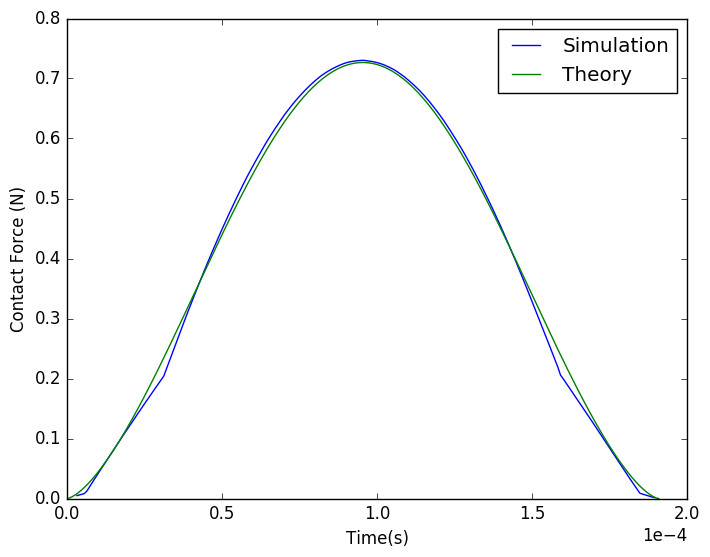
\includegraphics[width=0.55\textwidth]{{../images/force/Force-vel1.0}.png}
\label{fig:force1}
}
\subfloat[Velocity 0.10m/s]{
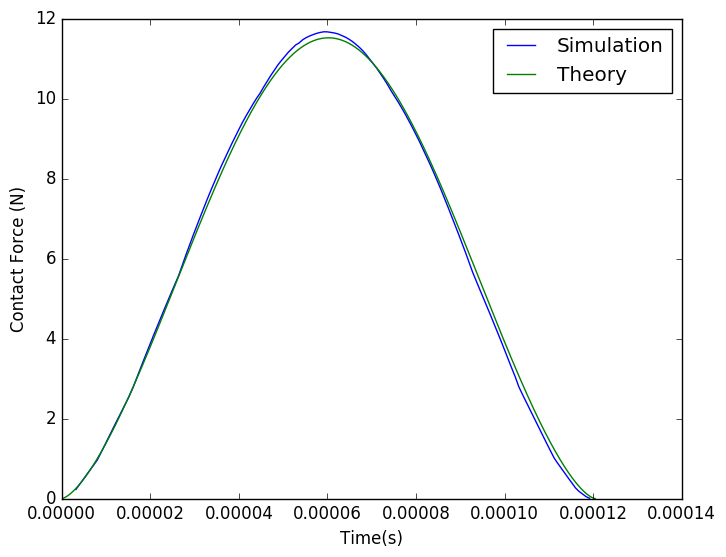
\includegraphics[width=0.55\textwidth]{{../images/force/Force-vel10.0}.png}
\label{fig:force10}
}

\subfloat[Velocity 0.20m/s]{
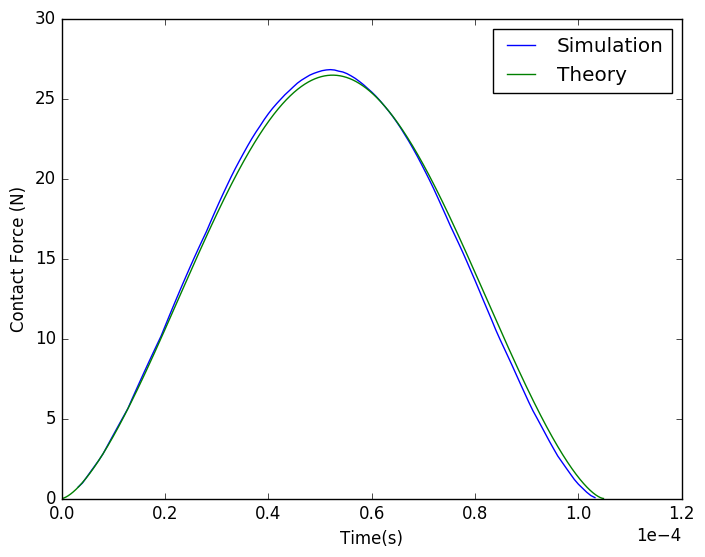
\includegraphics[width=0.55\textwidth]{{../images/force/Force-vel20.0}.png}
\label{fig:force20}
}
\subfloat[Velocity 0.30m/s]{
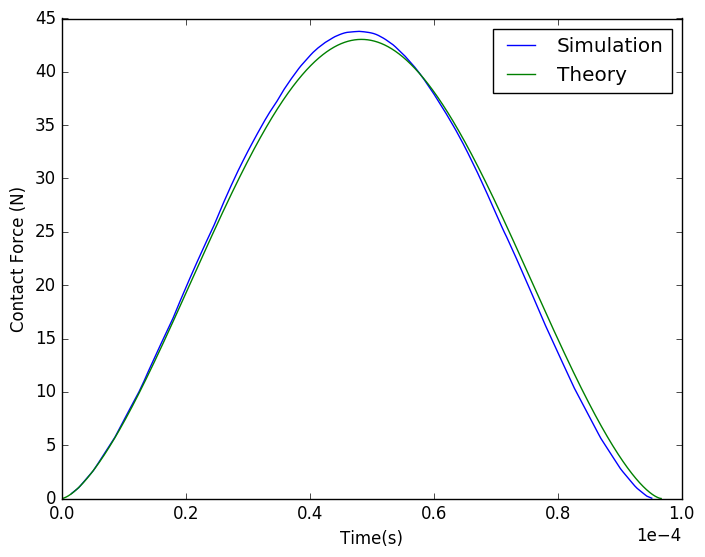
\includegraphics[width=0.55\textwidth]{{../images/force/Force-vel30.0}.png}
\label{fig:force30}
}

\subfloat[Velocity 0.50m/s]{
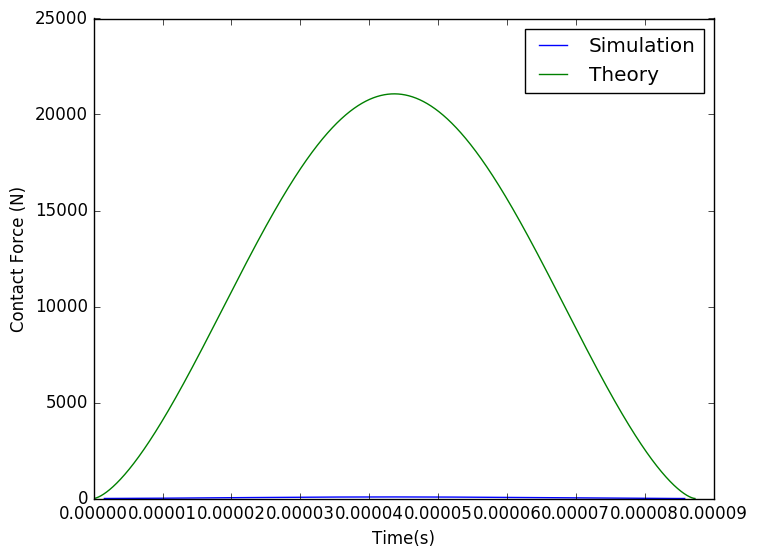
\includegraphics[width=0.55\textwidth]{{../images/force/Force-vel50.0}.png}
\label{fig:force50}
}
\subfloat[Velocity 3.0m/s]{
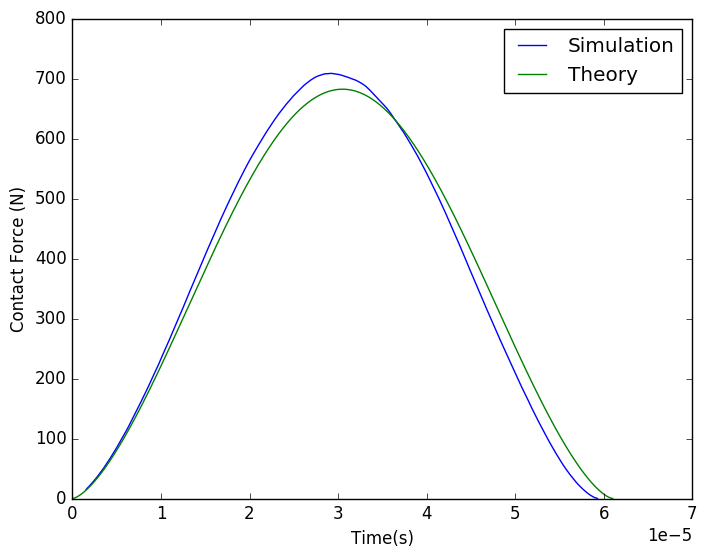
\includegraphics[width=0.55\textwidth]{{../images/force/Force-vel300.0}.png}
\label{fig:force300}
}
\caption{Contact force vs Time for various impact velocities}
\label{fig:force}
\end{figure}

The plots in \ref{fig:def} show the contact force between the sphere and the rigid plane. The plots shows that as the impact velocities are higher, the difference between the simulation data and the theoretical data is more visible. This errors is due the quasi static assumptions.


%%%%%%%%%%%%%%%%%%Energy%%%%%%%%%%%%%%%%%%%%


\subsection{Energy}
\begin{figure}[H]
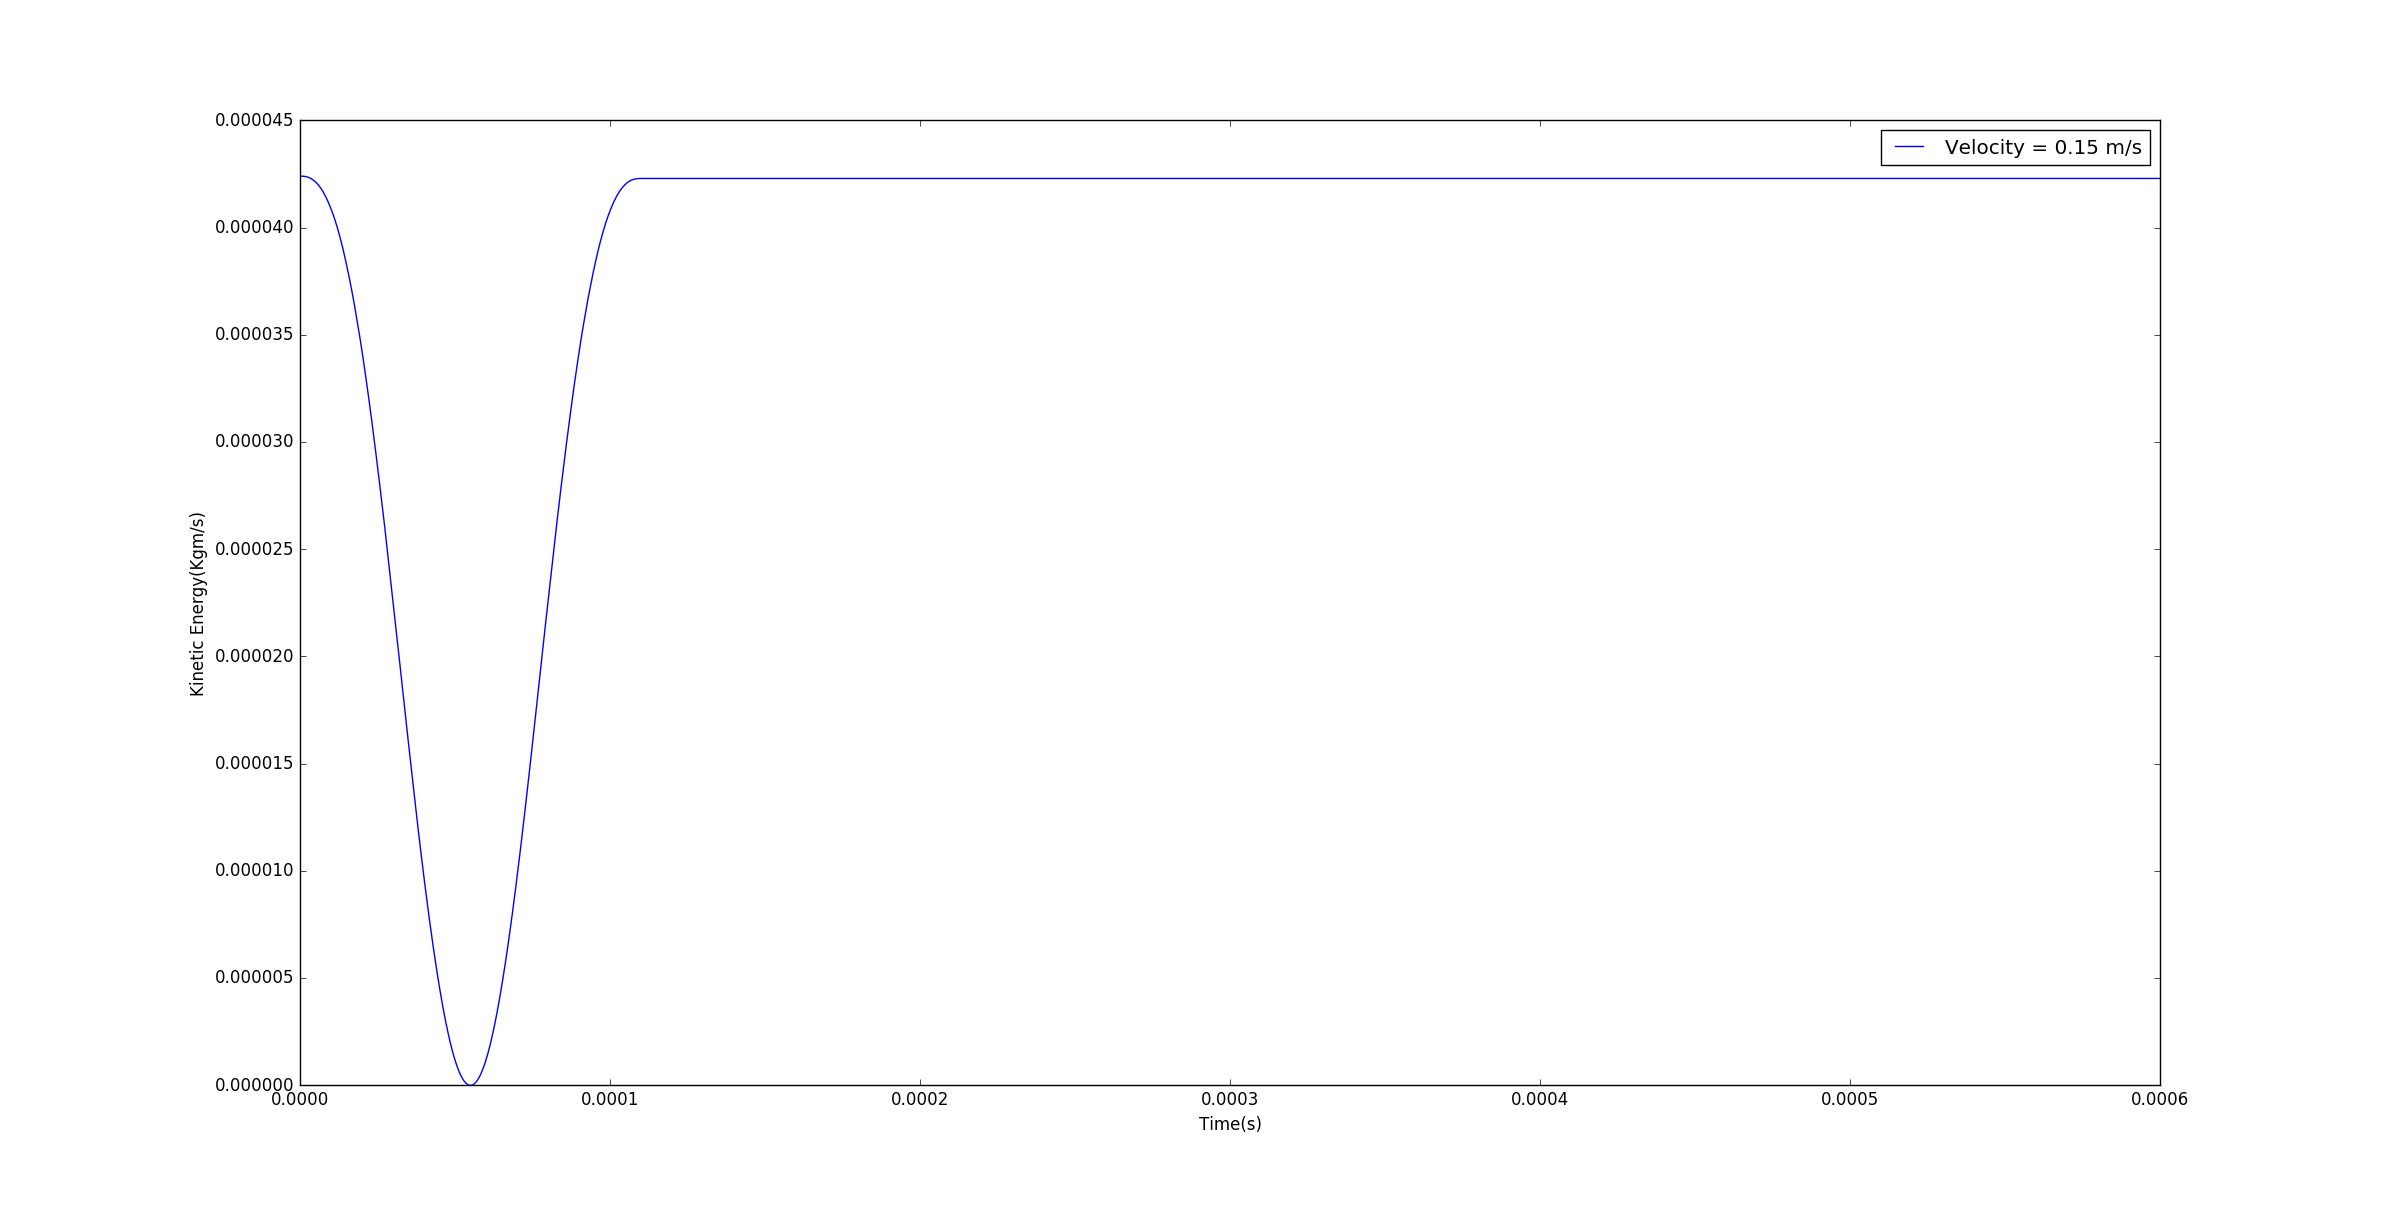
\includegraphics[width=1.0\textwidth]{../images/KE/KE.png}
\caption{Kinetic Energy}
\label{fig:KE}
\end{figure}
\begin{figure}[H]
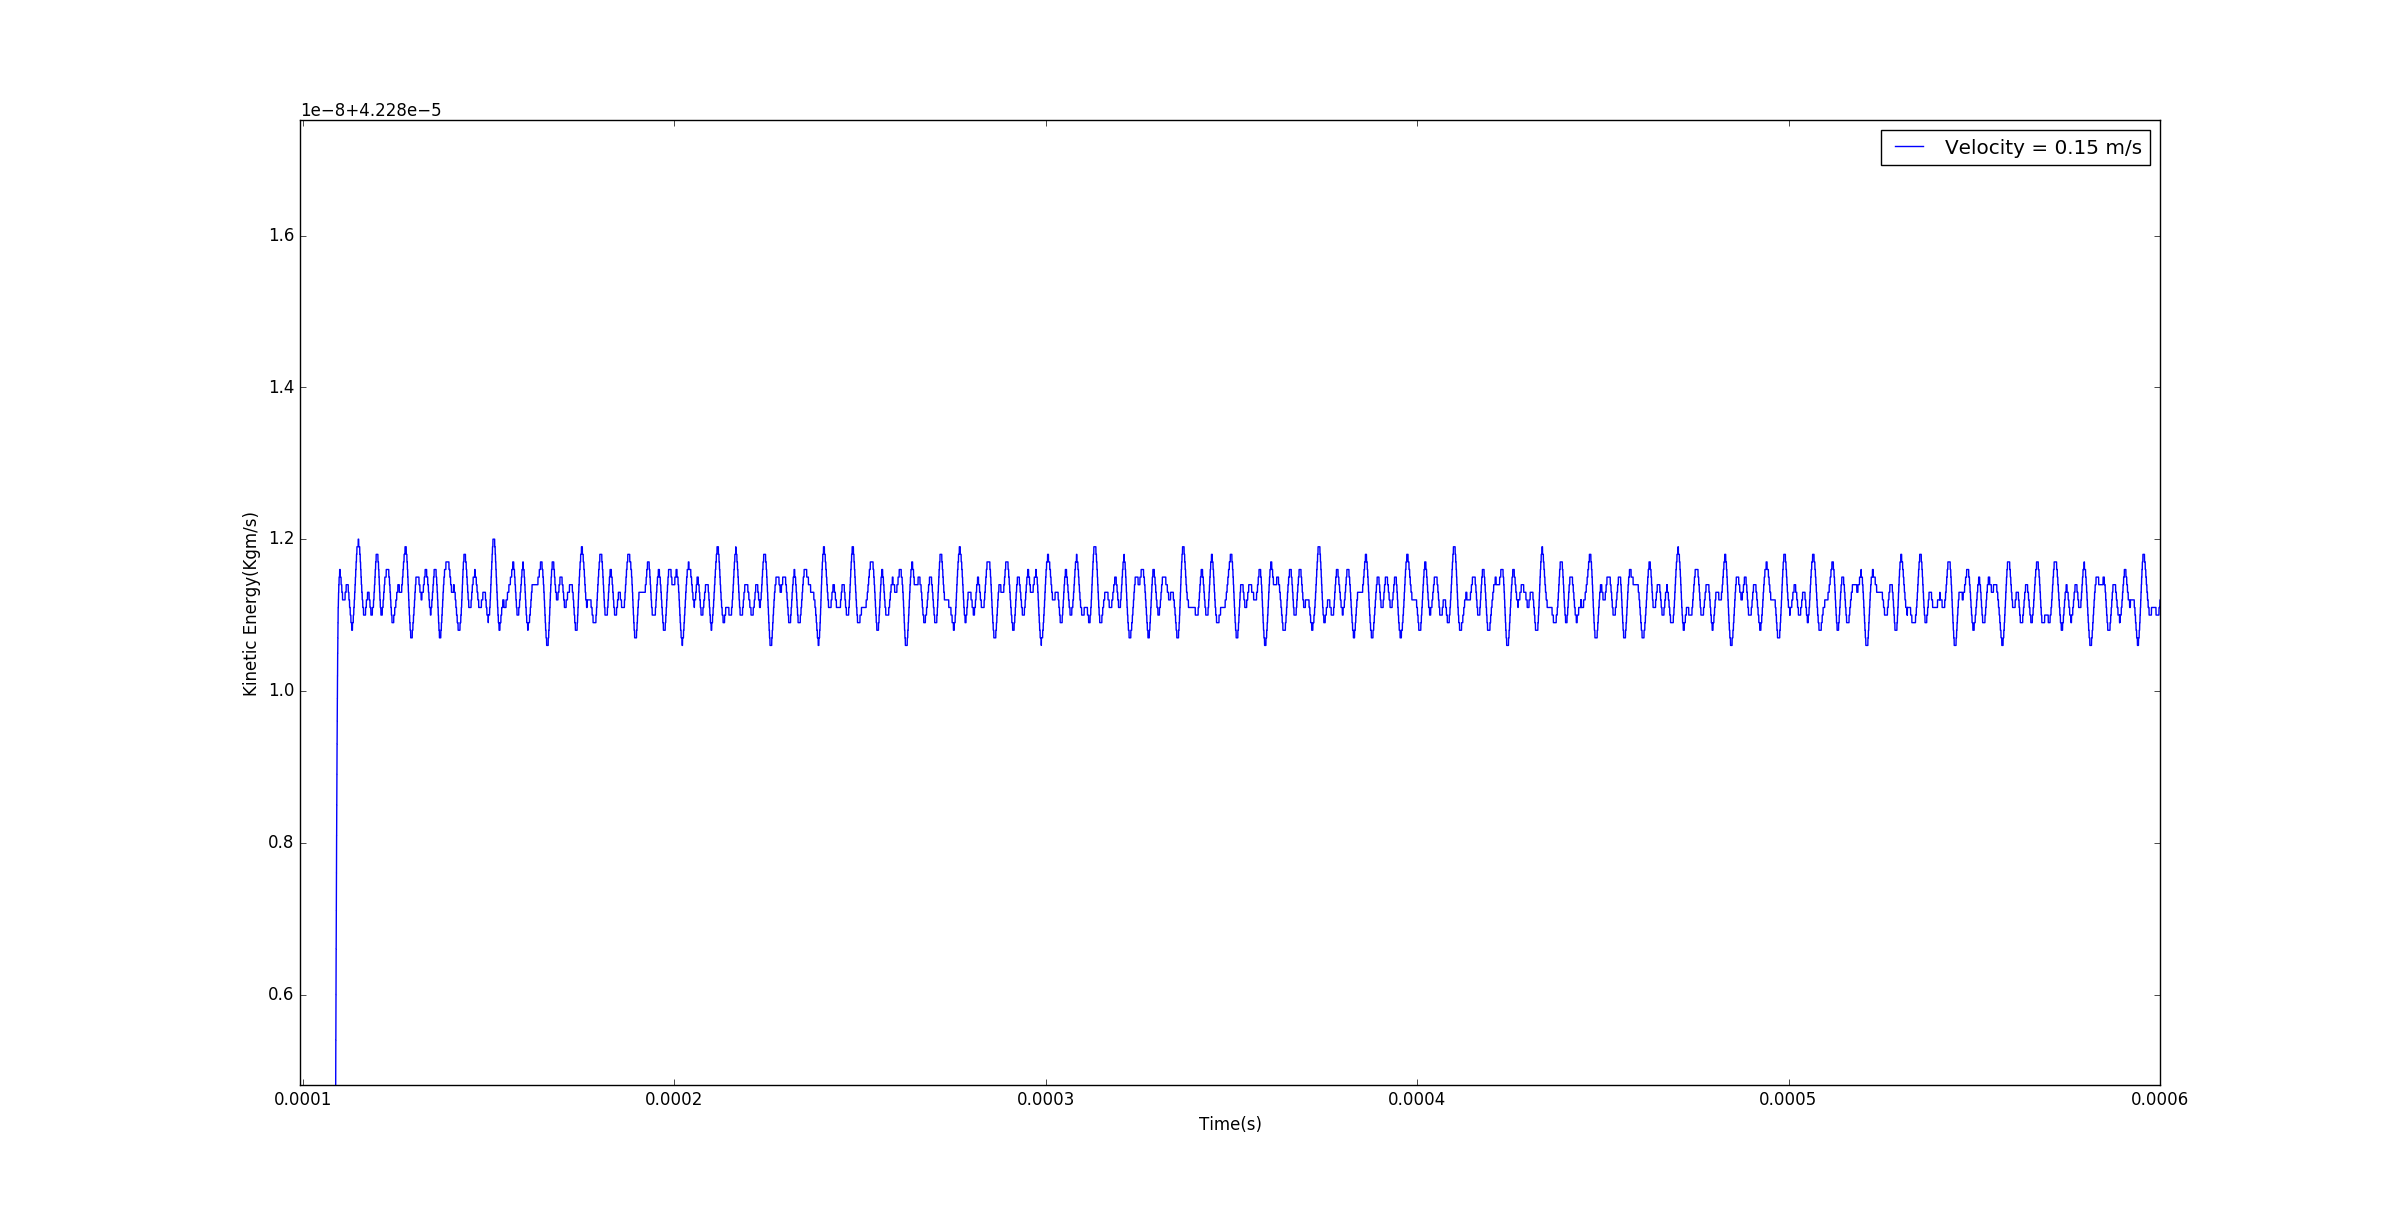
\includegraphics[width=1.0\textwidth]{../images/KE/KE-zoomed.png}
\caption{Kinetic Energy}
\label{fig:KEzoomed}
\end{figure}
Now considering a harder material, i.e. with $Youngs Modulus(E)$ of $9.3GPa$. This Youngs Modulus was chosen as it was neither to hard nor to soft and had the vibration visible. The figure \ref{fig:KE} shows Kinetic Energy vs Time for the impact velocity of $0.15m/s$. It is clear that the kinetic energy decreases in the beginning of the impact and increases towards the end of the impact. When observed carefully, fluctuations can be observed in the plot after the impact is completed as shows in \ref{fig:KEzoomed}. As disscussed in the previous paraghrah, this is because a part of the kinetic energy is converted into strain energy which cause vibrations in within the model.

A similar trend is also visible in the plot of the strain energy of the sphere. It is clear from \ref{fig:SEzoomed}, that after the collision is complete, the body still possesses a small amount of strain energy.

\begin{figure}[H]
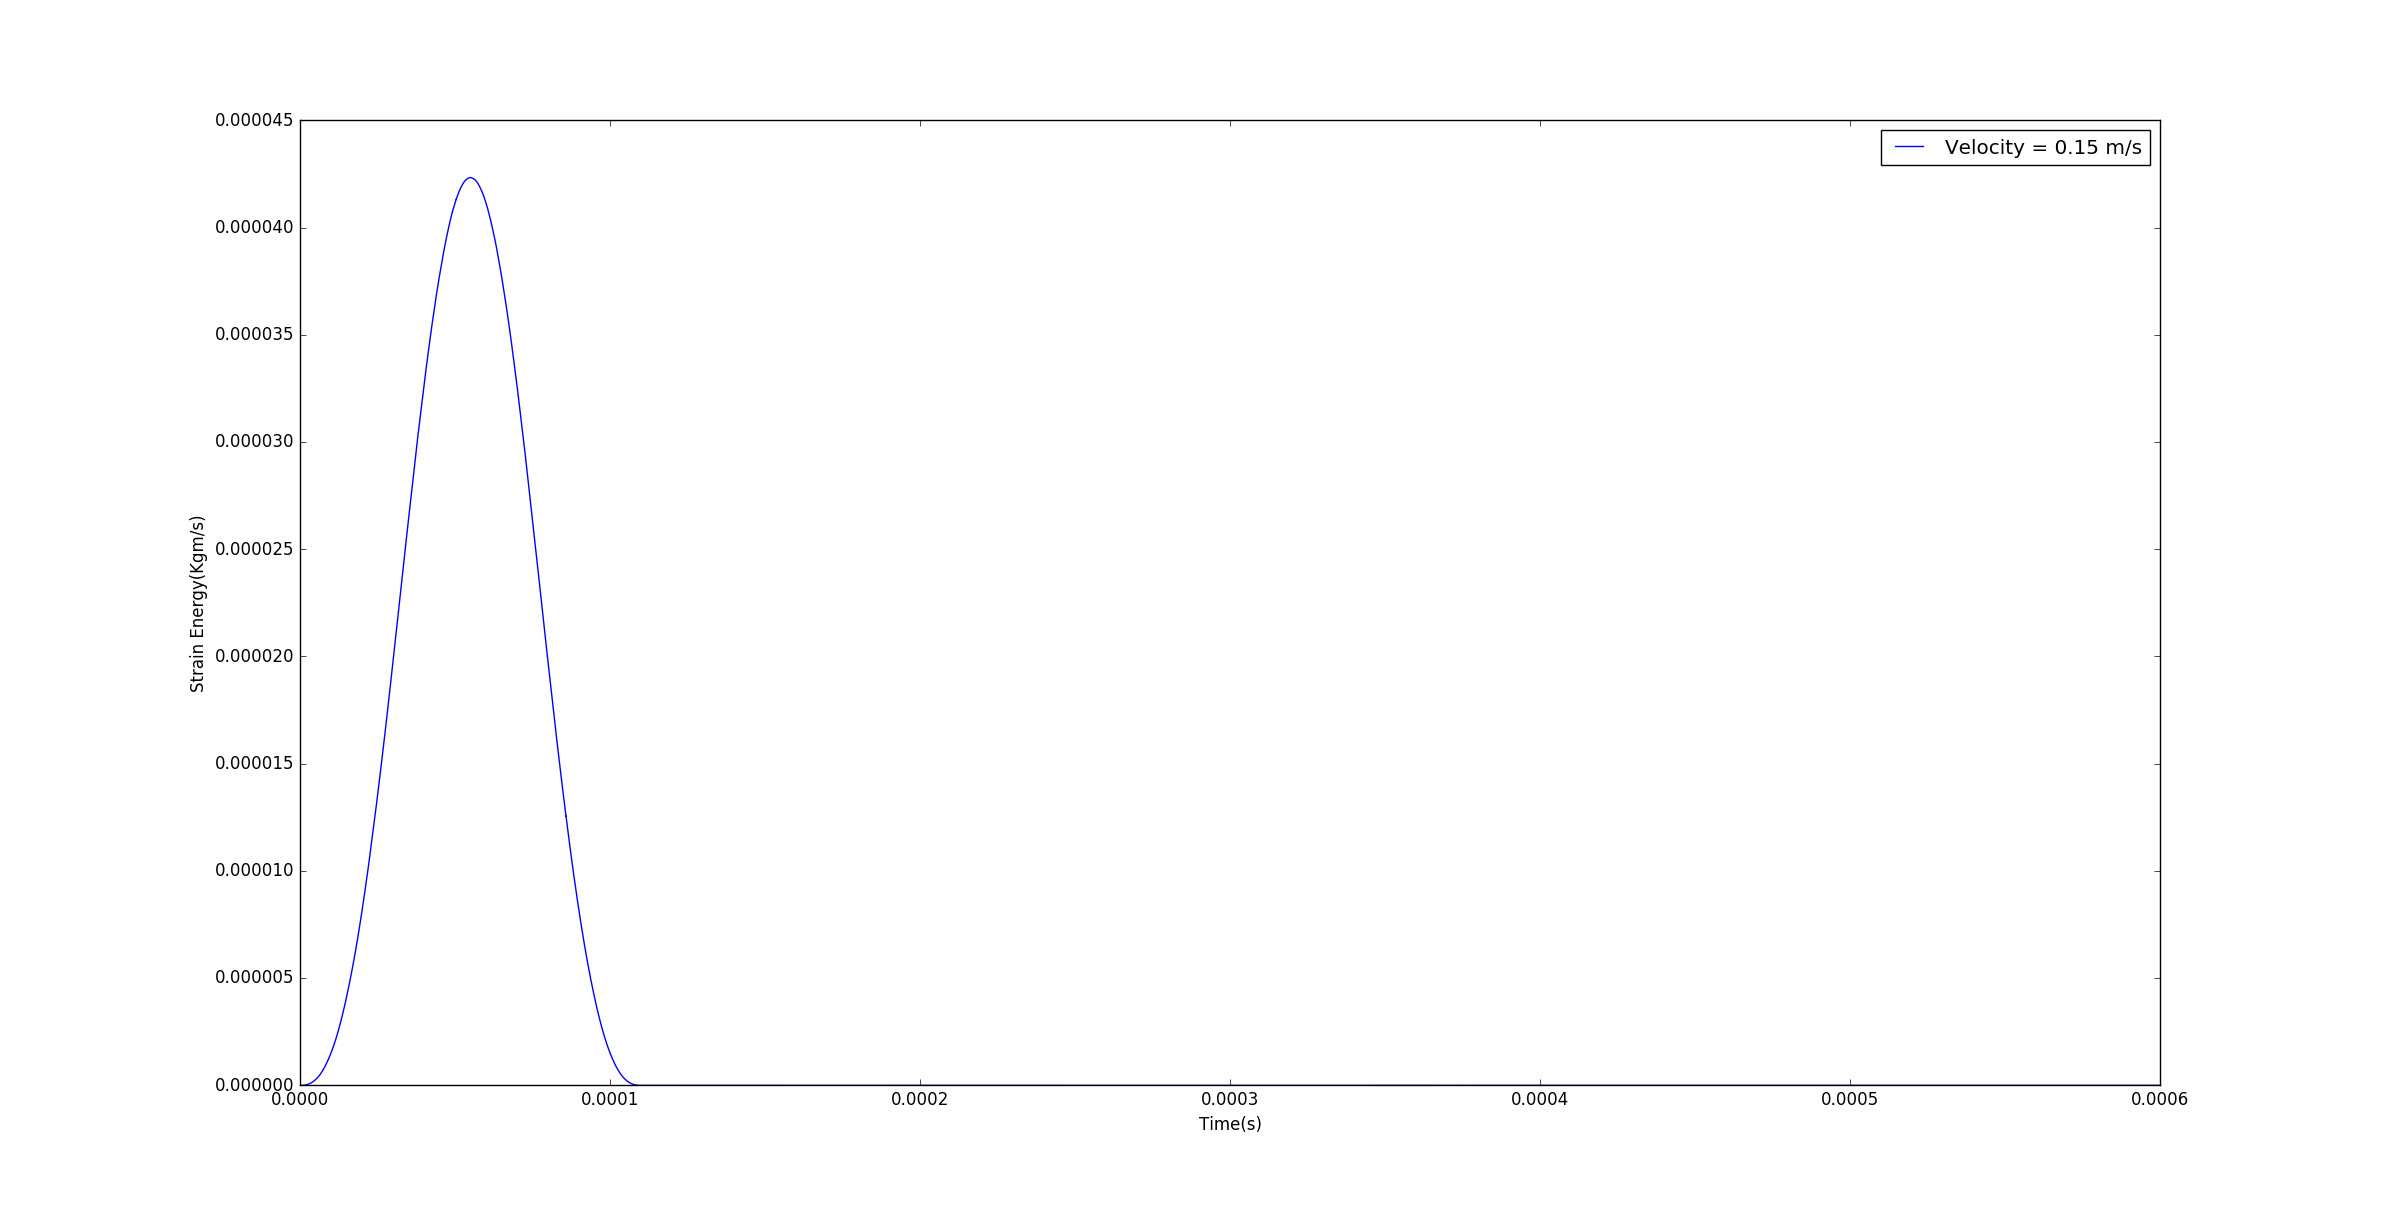
\includegraphics[width=1.0\textwidth]{../images/StrainEnergy/strainenergy.png}
\caption{Strain Energy}
\label{fig:SE}
\end{figure}
\begin{figure}[H]
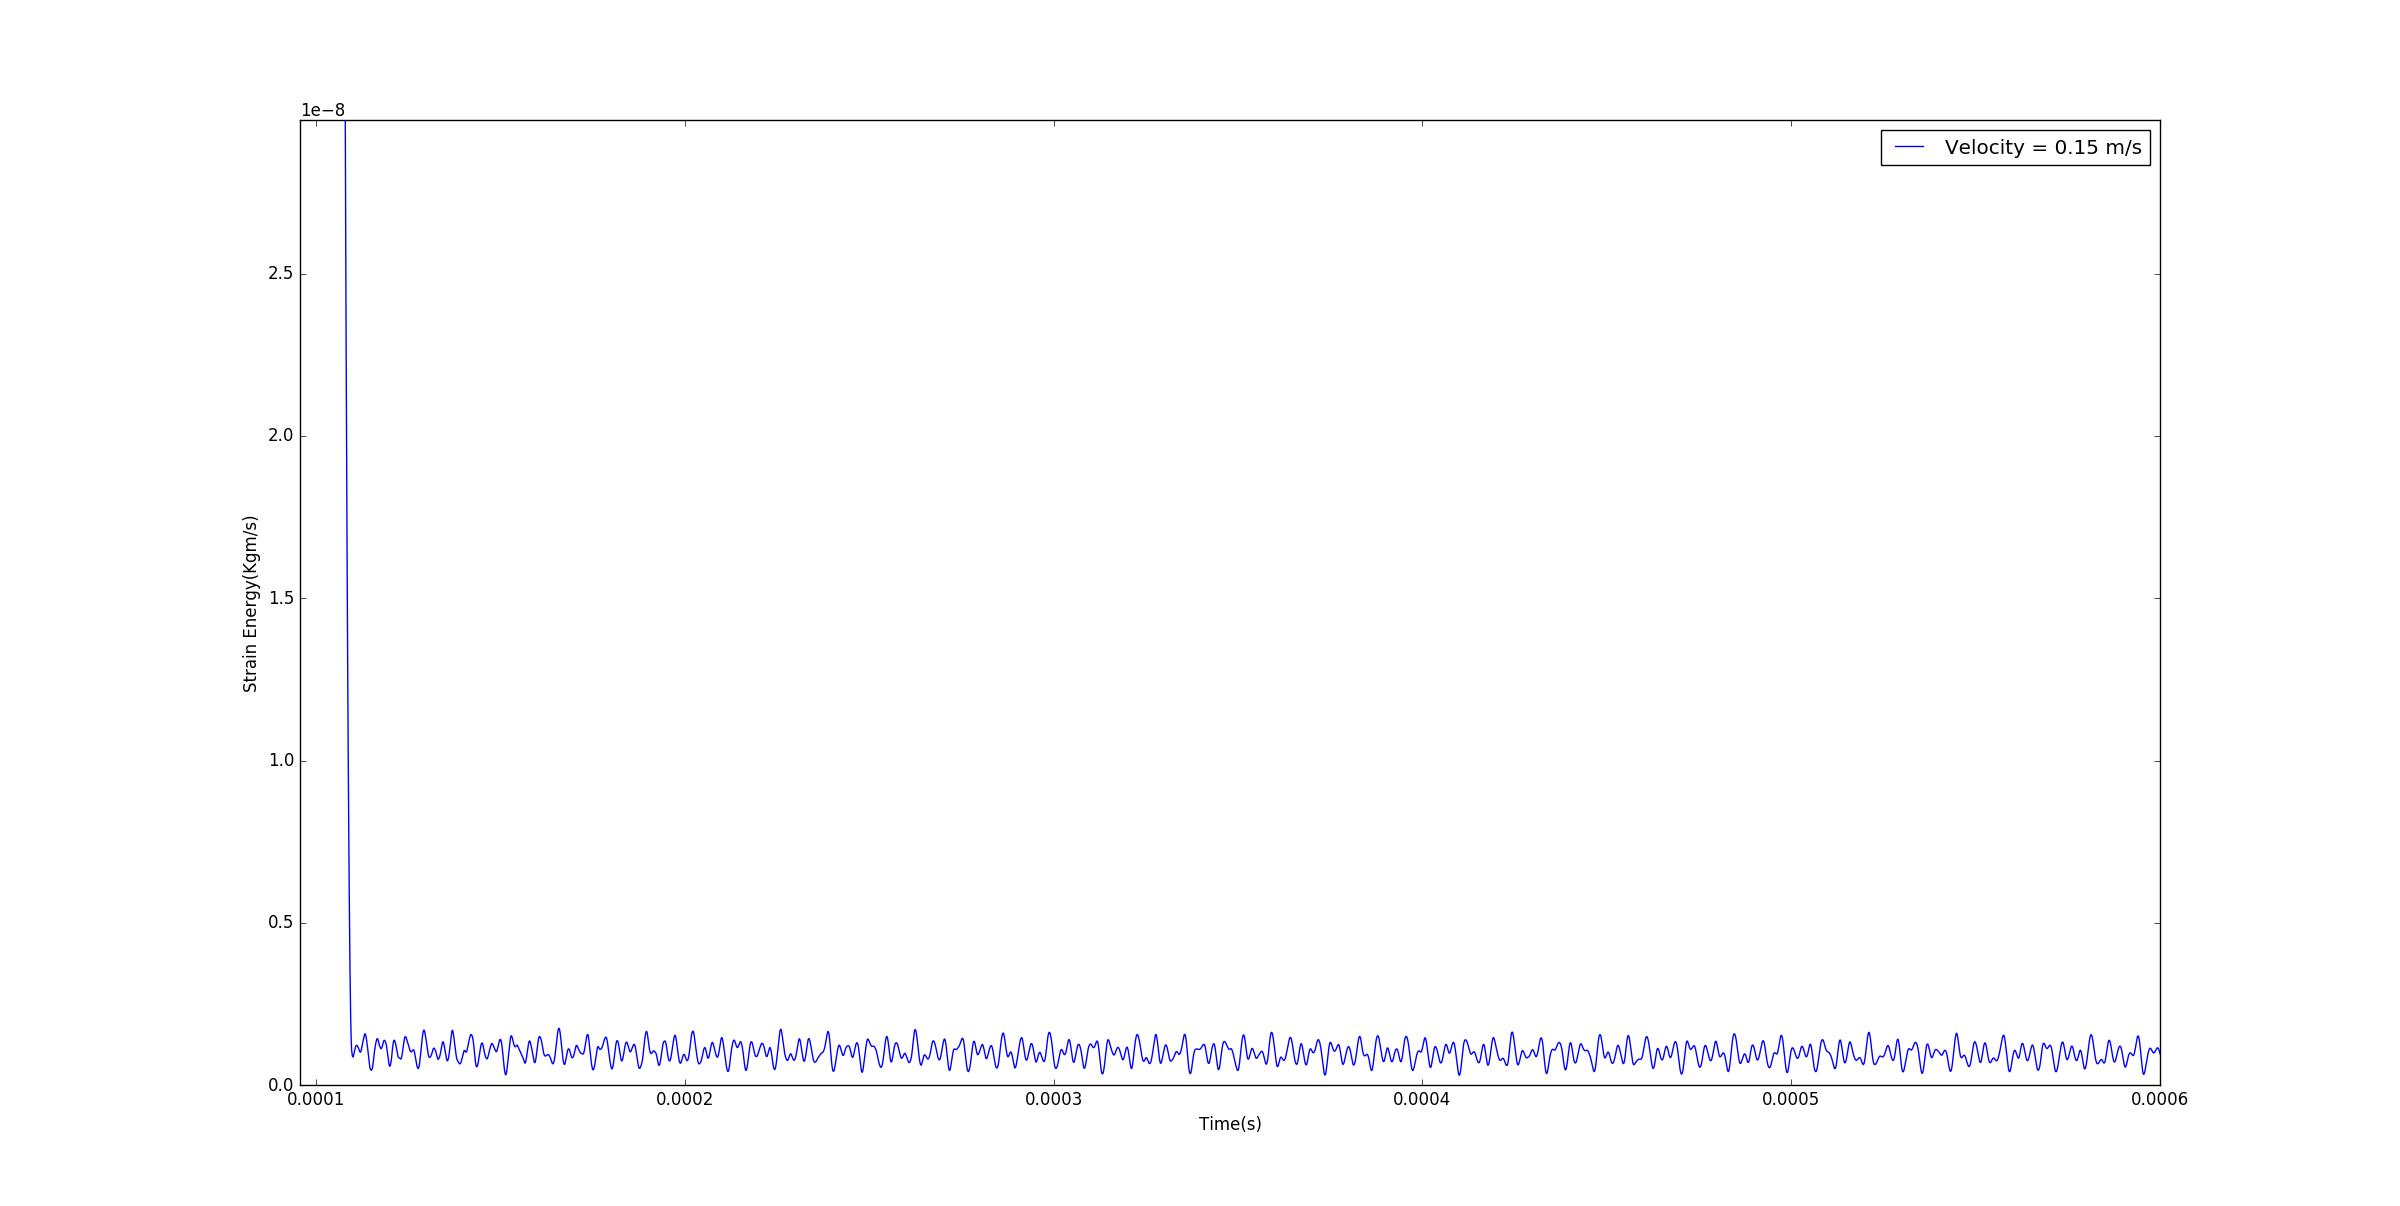
\includegraphics[width=1.0\textwidth]{../images/StrainEnergy/strainenergy-zoomed.png}
\caption{Strain Energy}
\label{fig:SEzoomed}
\end{figure}


\subsection{Co-efficient of Restitution}

\begin{figure}[H]
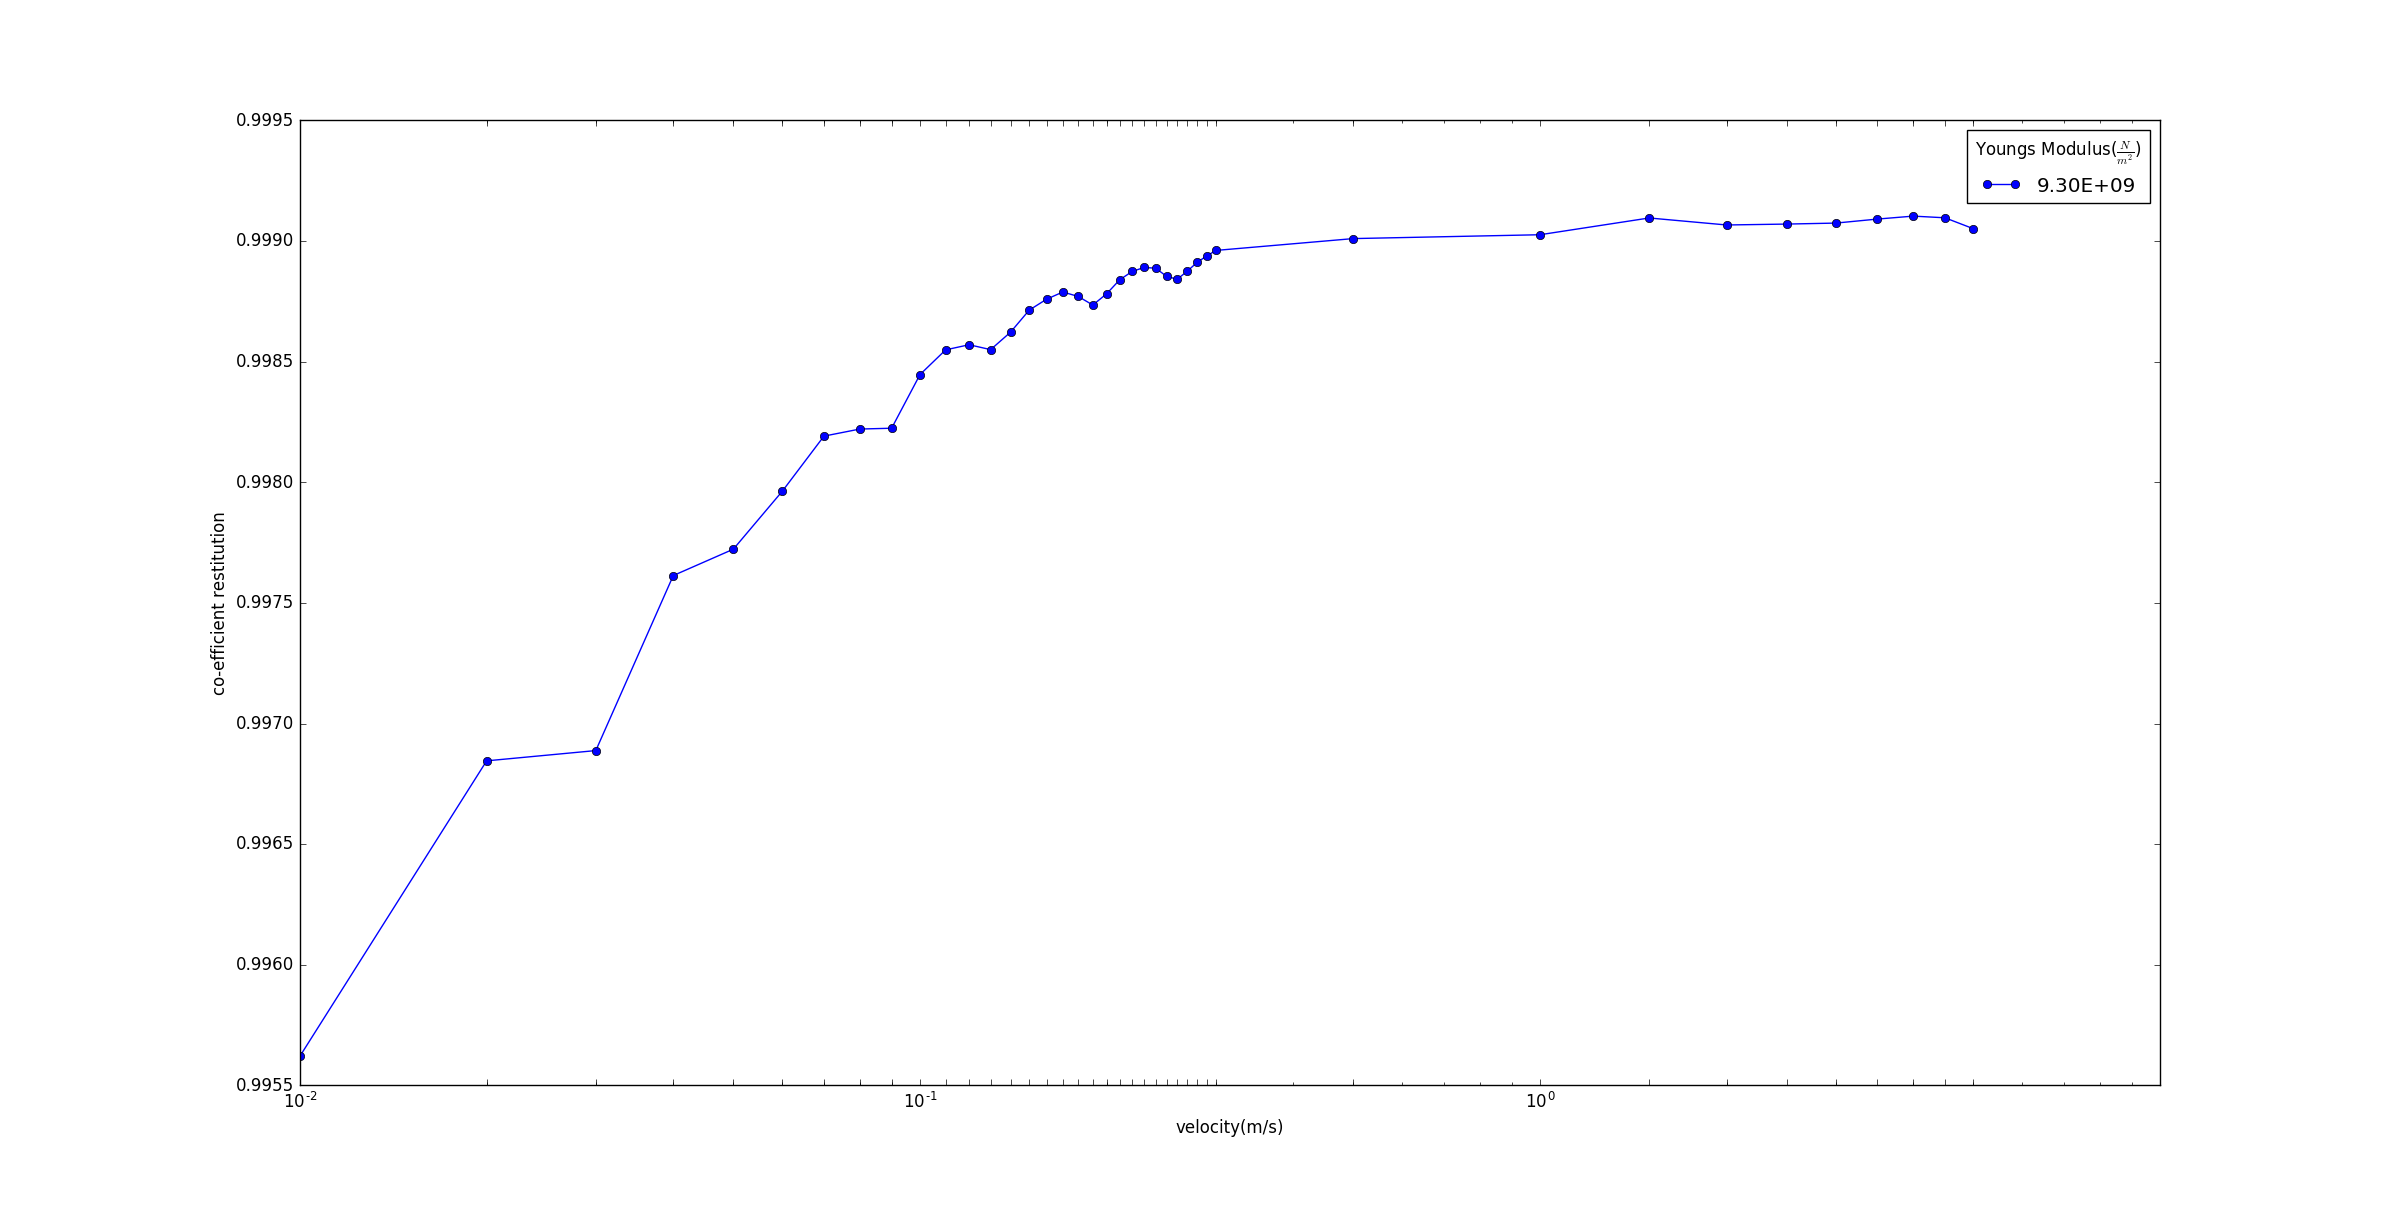
\includegraphics[width=1.0\textwidth]{../images/COR/COR.png}
\caption{co-efficient of restitution}
\label{fig:COR}
\end{figure}

To get a sense of the energy lost to vibrations, the co-efficient of restitution was calculate for an elastic material with $Youngs Modulus(E)$ of $9.3GPa$ and various impact velocities ranging from $0.01m/s to 5m/s$.
The co-efficient of restitution was calculated by,
\begin{equation}
COR = \sqrt{\frac{Kinetic\, Energy\, after\, impact}{Kinetic\, Energy\, before\, impact}}
\end{equation}
Kinetic Energy was used to calculate the co-efficient of restitution because, calculating trajectory of the center of mass of the model was much more computationally intensive and inaccurate than calculate the Kinetic energy of the complete.
Measure the co-efficient of restitution is a measure of the restitution of kinetic energy after the collision of two objects. The figure \ref{fig:COR} shows the co-efficient of restitution vs various impact velocities. We can see that the co-efficient of restitution increases as the impact velocities are increased. The bumps in the plot can be explained after performing a Fourier analysis on the models. The Fourier analysis shows that the bumps correspond to the eigen modes of the model.

\subsection{Modal Analysis}

To understand the plot \ref{fig:COR}, the modal analysis of the sphere was necessary. The natural frequencies of the sphere can affect the 

\section{Parametric Study}


%%%%%%%%%%%%%%%%%%%%%%%%%%%%%%%%%%%%%%%%%%%%



\subsection{Different Youngs Modulus}

\begin{figure}[H]
\subfloat[COR]{
\includegraphics[width=1.0\textwidth]{../images/parametricStudy/COR.png}
\label{fig:CORdiffE}
}
\end{figure}


\begin{figure}[H]
\subfloat[COR High Velocity]{
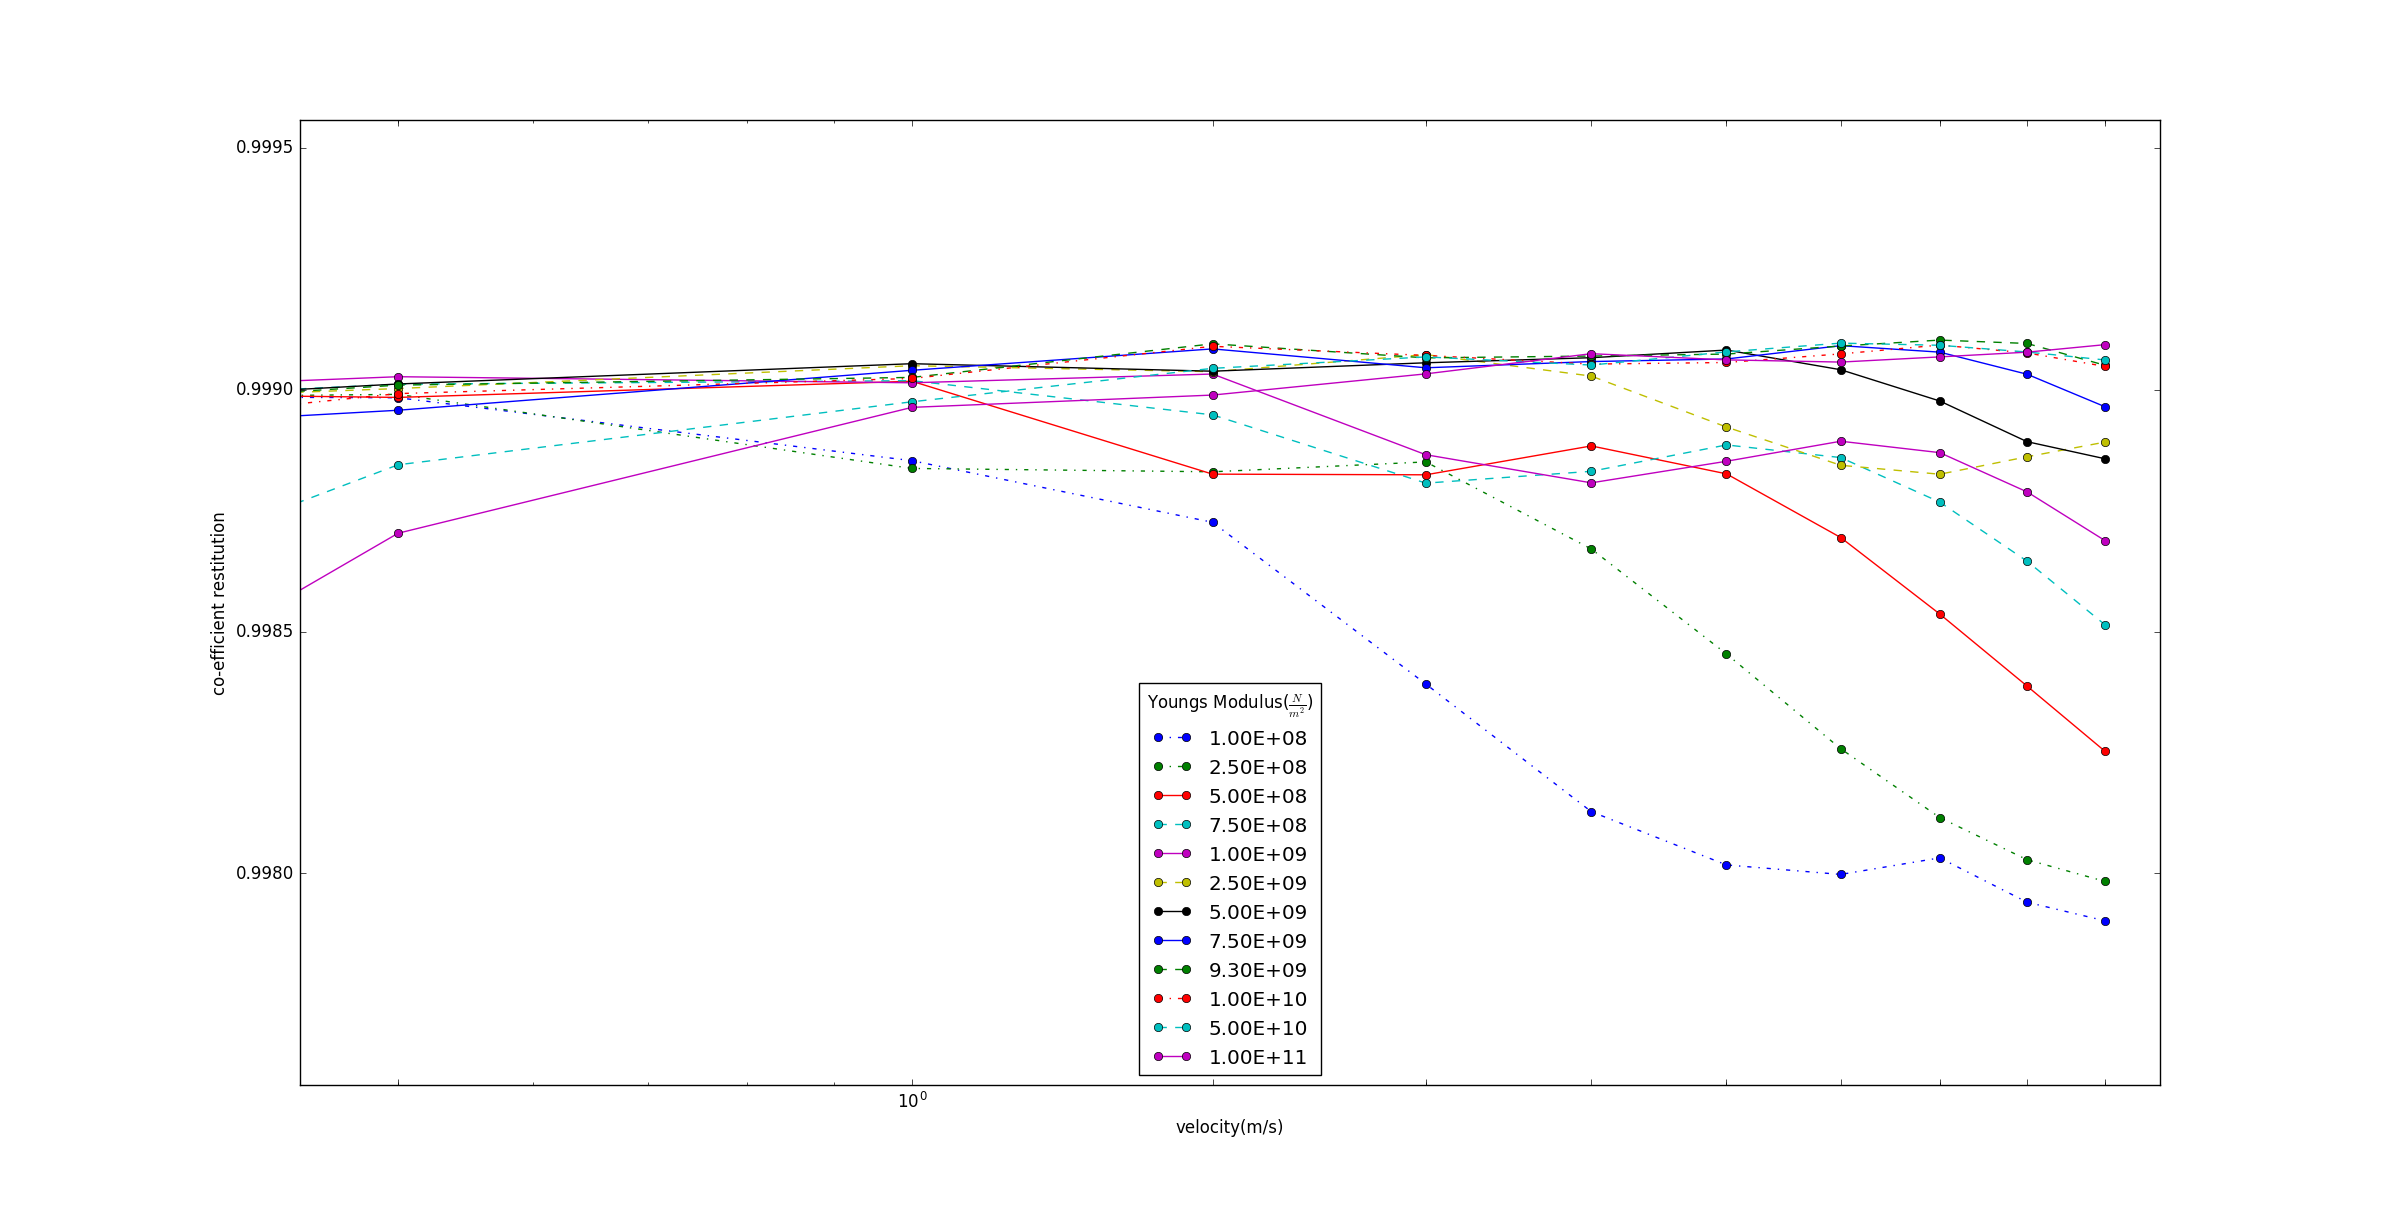
\includegraphics[width=0.55\textwidth]{../images/parametricStudy/COR_higherVEL.png}
\label{fig:CORdiffEHigh}
}
\subfloat[COR Low Velocity]{
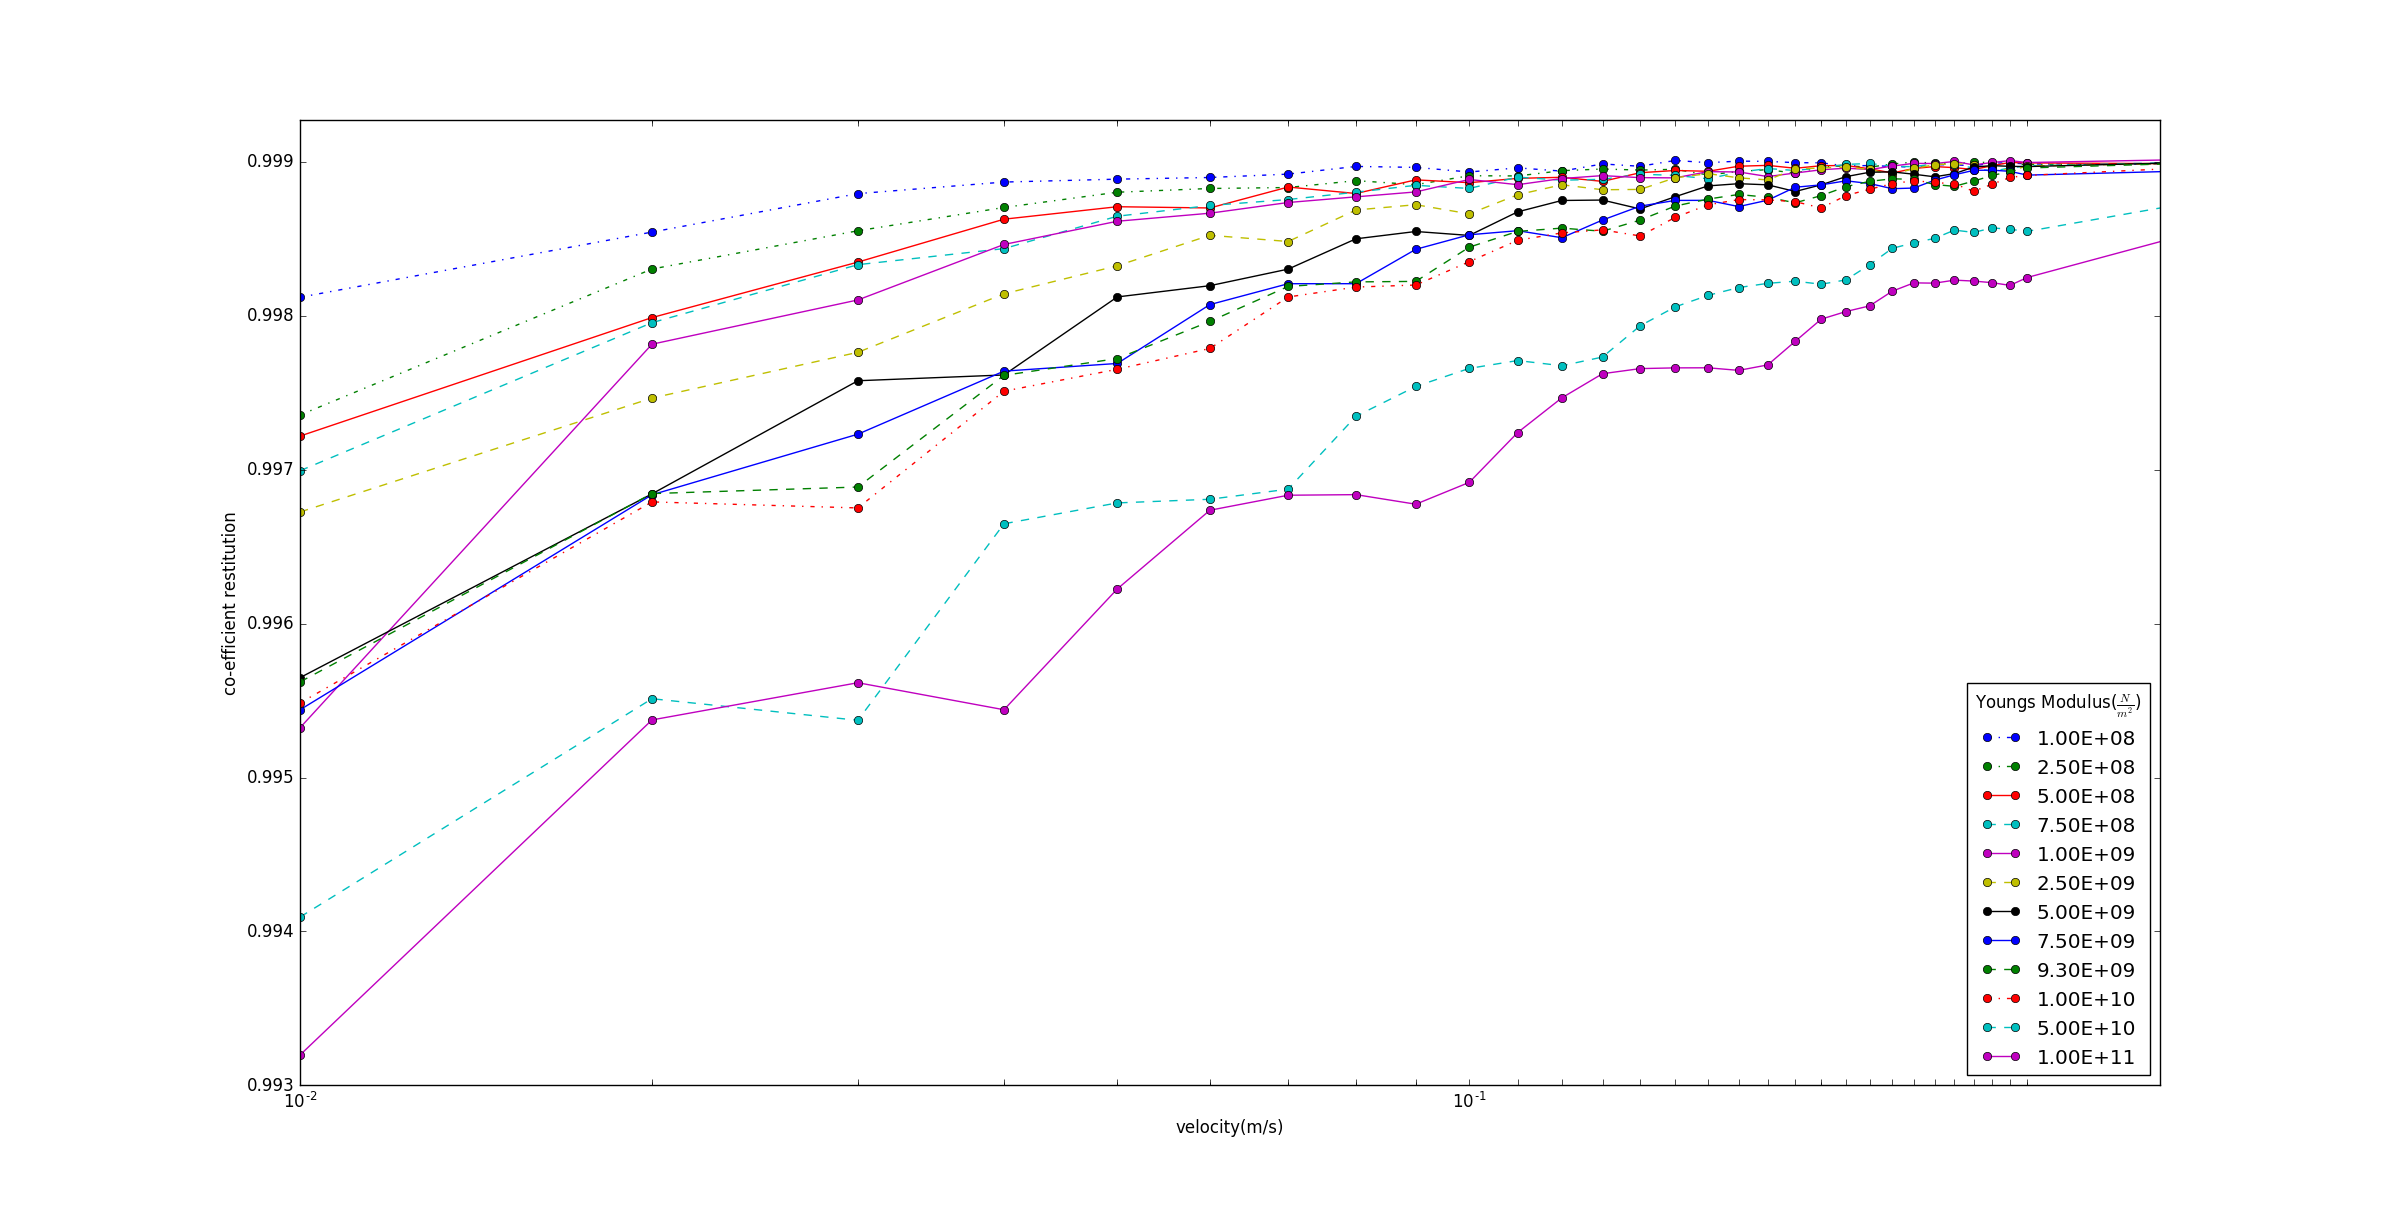
\includegraphics[width=0.55\textwidth]{../images/parametricStudy/COR_lowerVEL.png}
\label{fig:CORdiffELow}
}
\end{figure}


%%%%%%%%%%%%%%%%%%%%%%%%%%%%%%%%%%%%%%%%%%%%


\subsection{Different Diameters}

\begin{figure}[H]
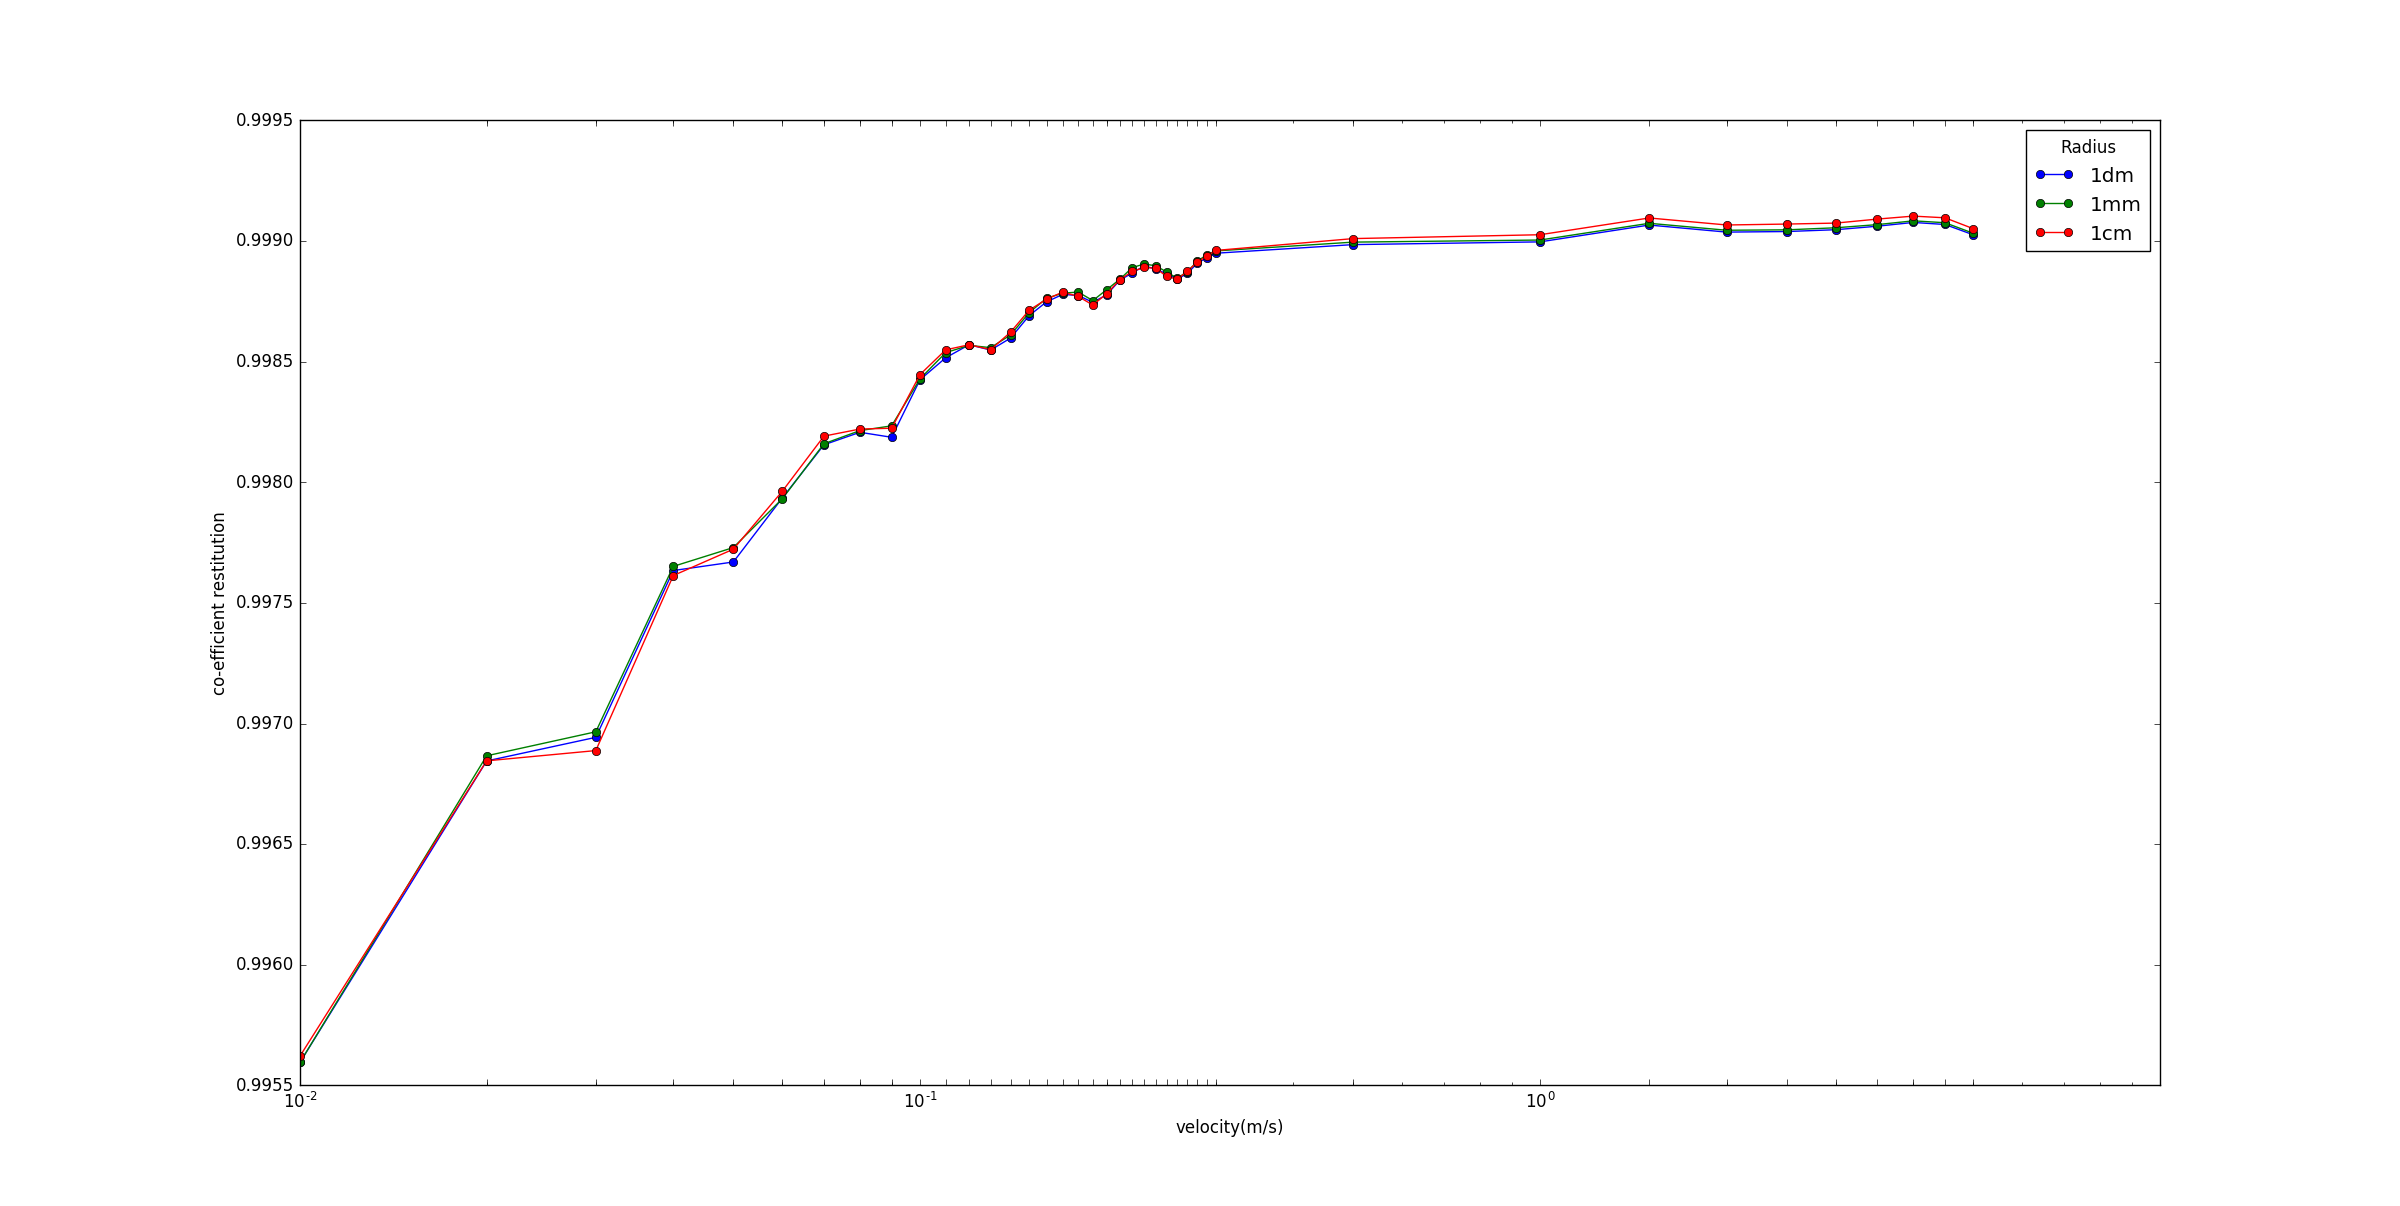
\includegraphics[width=1.0\textwidth]{../images/parametricStudy/CORvsVELdiffDAI.png}
\caption{COR}
\label{fig:CORDiffDia}
\end{figure}



%%%%%%%%%%%%%%%%%%%%%%%%%%%%%%%%%%%%%%%%%%%%



